\newpage
% ============================================================
%  SECTION: Results and Analysis
% ============================================================
\newpage
\section{Results and Analysis}
\label{sec:results}

This chapter presents the empirical findings of the data-safety experiment. To isolate the mechanical differences between native Kubernetes scaling and operator-driven scaling, the evaluation was conducted under quiescent conditions (zero external write pressure). A deterministic baseline was established for both scenarios: a Redis Cluster deployed with four primary master nodes and exactly \num{5000} keys uniformly distributed across the keyspace. The independent variable is the mechanism used to scale the cluster inward from four masters to three.

\subsection{Scenario A: Native HPA Scale-In and the Data Cliff}
\label{subsec:results-hpa}

In the native Horizontal Pod Autoscaler (HPA) scenario, the scaling action was triggered by directly reducing the \texttt{StatefulSet} replica count from four to three. This mirrors the exact operational instruction an HPA controller issues when resource utilisation falls below its target threshold.

Because Kubernetes \texttt{StatefulSets} terminate pods in strictly descending ordinal order (\cite{k8s_statefulsets}), the scheduler immediately issued a termination signal to the highest-ordinal pod (\texttt{redis-3}). The native Kubernetes primitives possess no awareness of the Redis hash slot topology; consequently, the pod was terminated without initiating a \texttt{CLUSTER MEET} or migrating its assigned hash slots to the surviving nodes.

As recorded in the test output, the instantaneous removal of \texttt{redis-3} triggered a catastrophic data cliff:
\begin{itemize}
    \item \textbf{Slot Orphanage:} Cluster hash slot coverage fell immediately from \num{16384} to \num{12288}, leaving \num{4096} slots permanently orphaned.
    \item \textbf{Data Loss:} The total key count dropped from \num{5000} to \num{3750}. Exactly \num{1250} keys (25\% of the dataset, correlating directly to the loss of one out of four evenly balanced nodes) were permanently deleted.
    \item \textbf{Availability:} The read probes executed immediately following the pod deletion resulted in a 100\% failure rate. Because the cluster fell below the full \num{16384} slot coverage requirement, Redis transitioned into a \texttt{CLUSTERDOWN} state, refusing all subsequent read and write traffic (\cite{redis_cluster_spec}).
\end{itemize}

These results validate the hypothesis that native Kubernetes scaling primitives provision and terminate compute capacity but are structurally incapable of integrating or safely decommissioning stateful topology. 


\begin{figure}
    \centering
    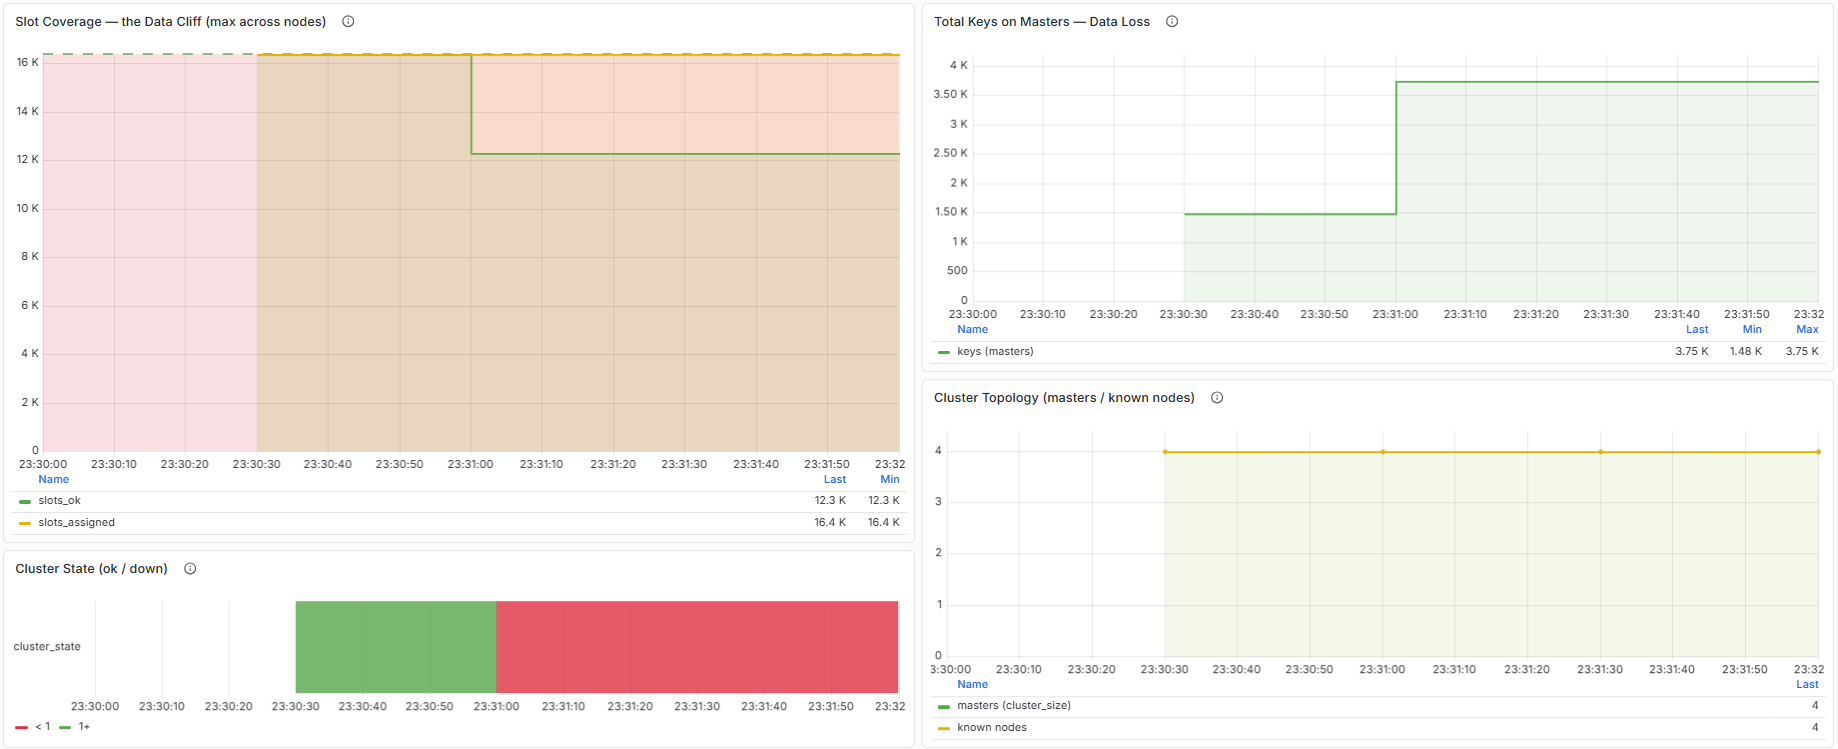
\includegraphics[width=\textwidth]{assets/images/hpa_scale_in.png}
    \caption{Timeline of the HPA scale-in event. The vertical red line indicates the moment the \texttt{StatefulSet} replica count was reduced from four to three, triggering the deletion of \texttt{redis-3}. The subsequent drop in total keys and hash slot coverage is visible, along with the spike in read errors due to cluster unavailability.}
    \label{fig:hpa_scale_in}
\end{figure}


\subsection{Scenario B: Operator-Driven Graceful Scale-In}
\label{subsec:results-operator}

In the operator scenario, the scale-in was executed by patching the \texttt{clusterSize} parameter of the \texttt{RedisCluster} Custom Resource from four down to three. This mirrors the exact action taken by a KEDA \texttt{ScaledObject} triggering a downscale event.

Rather than immediately terminating a pod, the Opstree Redis Operator intercepted the state change. The operator's reconciliation loop identified the required topological shift and initiated a live resharding process, draining the \num{4096} hash slots from the target node and redistributing them evenly among the three surviving masters (\cite{opstree_redis}). Only after the cluster achieved consensus that the departing node held zero slots did the operator delete the underlying \texttt{StatefulSet} pod.

The test output confirms a fully graceful scale-in:
\begin{itemize}
    \item \textbf{Slot Integrity:} Hash slot coverage remained at \num{16384} throughout and after the scaling event.
    \item \textbf{Data Preservation:} The cluster retained all \num{5000} keys with zero data loss.
    \item \textbf{Availability:} The read probes executed following the scale-in recorded zero \texttt{CLUSTERDOWN} errors, confirming that cluster availability was maintained continuously. 
\end{itemize}

\subsection{Synthesis of Findings}
\label{subsec:results-synthesis}

The stark contrast between the two scenarios empirically proves the necessity of the operator pattern for stateful workloads. The native HPA pathway demonstrates that allowing a generic infrastructure controller to manage database lifecycle operations results in guaranteed data loss and cluster unavailability. 

While the operator successfully bridged the gap between compute provisioning and data topology, it is important to note that this success was recorded under quiescent conditions. As established in the methodology, the operator's live resharding logic remains vulnerable to interruption if subjected to heavy concurrent write pressure (\cite{redis_admin}). Nevertheless, when evaluating pure architectural capability, the operator pattern is the only evaluated mechanism that possesses the domain knowledge required to safely perform a stateful scale-in.

\begin{figure}
    \centering
    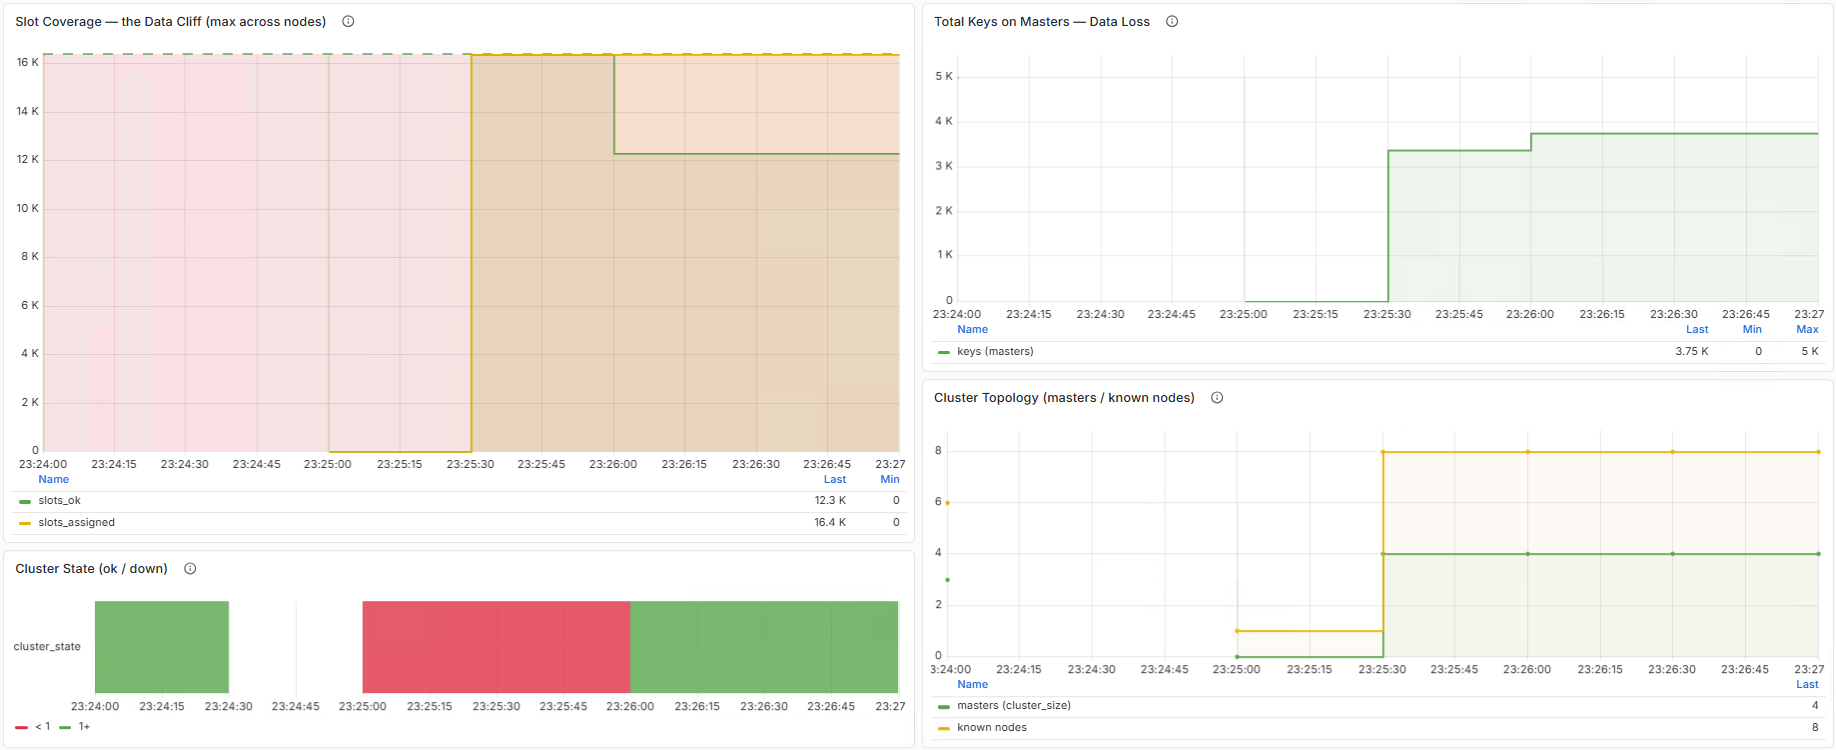
\includegraphics[width=\textwidth]{assets/images/operator_scale_in.png}
    \caption{Timeline of the operator-driven scale-in event. The vertical blue line indicates the moment the \texttt{clusterSize} parameter was patched from four to three. The graph shows that total keys and hash slot coverage remained stable throughout the resharding process, and no read errors were recorded, confirming continuous availability.}
    \label{fig:operator_scale_in}
\end{figure}